%% Version 4.3.2, 25 August 2014
%
%%%%%%%%%%%%%%%%%%%%%%%%%%%%%%%%%%%%%%%%%%%%%%%%%%%%%%%%%%%%%%%%%%%%%%
% Template.tex --  LaTeX-based template for submissions to the 
% American Meteorological Society
%
% Template developed by Amy Hendrickson, 2013, TeXnology Inc., 
% amyh@texnology.com, http://www.texnology.com
% following earlier work by Brian Papa, American Meteorological Society
%
% Email questions to latex@ametsoc.org.
%
%%%%%%%%%%%%%%%%%%%%%%%%%%%%%%%%%%%%%%%%%%%%%%%%%%%%%%%%%%%%%%%%%%%%%
% PREAMBLE
%%%%%%%%%%%%%%%%%%%%%%%%%%%%%%%%%%%%%%%%%%%%%%%%%%%%%%%%%%%%%%%%%%%%%

%% Start with one of the following:
% DOUBLE-SPACED VERSION FOR SUBMISSION TO THE AMS
\documentclass{ametsoc}

% TWO-COLUMN JOURNAL PAGE LAYOUT---FOR AUTHOR USE ONLY
% \documentclass[twocol]{ametsoc}

%%%%%%%%%%%%%%%%%%%%%%%%%%%%%%%%
%%% To be entered only if twocol option is used

\journal{jpo}


%%%%%%%%%%%%%%%%%%%%%%%%%%%%%%%%
%Citations should be of the form ``author year''  not ``author, year''
\bibpunct{(}{)}{;}{a}{}{,}

\title{Diagnosing the Influence of Mesoscale Eddy Fluxes on the Deep Western Boundary Current in the 1/10$^\circ$ STORM / NCEP Simulation}

\authors{Veit L\"uschow \correspondingauthor{Max-Planck Institute for Meteorology, Bundesstraße 53, Hamburg, Germany}}

%% Follow this form:
    % \affiliation{American Meteorological Society, 
    % Boston, Massachusetts.}

\affiliation{}

\email{veit.lueschow@mpimet.mpg.de}

%% If appropriate, add additional authors, different affiliations:
    \extraauthor{Jin-Song von Storch}
    \extraauthor{Jochem Marotzke}
    %\extraaffil{Affiliation, City, State/Province, Country}

%%%%%%%%%%%%%%%%%%%%%%%%%%%%%%%%%%%%%%%%%%%%%%%%%%%%%%%%%%%%%%%%%%%%%
% ABSTRACT

\abstract{Enter the text of your abstract here.}

\begin{document}
\maketitle


\section{Introduction}


The common picture of the meridional overturning circulation being an \textit{ocean conveyor belt} \citep{Broecker1991} assumes that the deep western boundary current (DWBC) carries a large fraction of the North Atlantic deep water (NADW) from the deep convection sites in the Labrador and Nordic seas, along the East American shoreline, to the South. Yet, findings of interior pathways for NADW towards the South call into question whether the DWBC is the only route to close the meridional overturning in this direction (see \citep{Lozier2010} for a review). Trajectories of Eulerian floats released near the NADW formation sites suggest significant detrainment and entrainment of DWBC water with the surrounding interior waters via mesoscale eddies \citep{Fischer2002, Bower2009}. However, even if the DWBC is not a continuous pathway for NADW, ocean models and observations agree that it plays an important role in balancing the upper ocean northward flow  (Lumpkin and Speer 2007??). In this function, the DWBC is relevant for the meridional exchange of heat in the Atlantic region.\\
\citet{Stommel1959} first proposed a theory on the existence of deep boundary currents like the DWBC more than 50 years ago - a few years before it was actually observed by \citet{Swallow1961}. Since then, the DWBC has received less attention then its northward flowing counter part in the upper ocean (review paper?) that provides Northern Europe with relatively warm climate. Existing studies dealing with the DWBC mostly focus on its temporal variability and relate that to  Rossby wave signals \citep{Boning} (Bryden???) or changes in the wind stress curl over the North Atlantic \citep{Lee1996}. \citet{Dengler2004} and \citet{Schott2005} investigate the structure of the DWBC south of the equator and find that it breaks up into eddies at 8$^\circ$S. 

\begin{itemize}
\item give paper overview:
\begin{enumerate}
\item descriptive part
\item comparison with observations
\end{enumerate}
\end{itemize}
\section{An eddying DWBC in the STORM Simulation} 
The STORM/NCEP Simulation represents the observed DWBC reasonably well in its mean meridional transport, lateral and vertical extension and meridional velocity magnitude. We show this exemplary by comparing the above mentioned characteristics with observations from 26.5$^\circ$N, where the DWBC has received much attention in observational studies since the late 1980s. Estimates of its time-averaged southward transport range from 11 Sv \citep{Meinen2006} to 40 Sv \citep{Lee1996}. This large spread originates in a large DWBC variability on different timescales (standard deviation of up to 20 Sv \citep{Bryden2005a}) as well as different observational setups. In our model, the effective southward DWBC transport at 26.5$^\circ$N is 13 Sv. This transport consists of a narrow and strong boundary current of 120 km width that accounts for 23 Sv \textit{southward} flow and an adjacent \textit{northward} recirculation of 10 Sv that extends to about 550 km offshore (Fig. \ref{fig:intro_dwbc_structure}).  Compared to recent observational studies by \citet{Meinen2013} and \citet{Johns2008} that use the RAPID array (references), the net transport in our model seems to be too low by a factor of about 1.5. However, the lateral and vertical extension of the flow, including the sign change in the meridional velocity at about 120 km offshore, the DWBC core depth (about 2000 m) and the maximum velocity in the core (about 0.2 m/s, Fig. \ref{fig:intro_dwbc_structure}) match observations \citep{Lee1996, Bryden2005a} quite well. Although the net transport in the STORM model seems to be too low compared to observations, it accounts for 80 \% of the southward transport necessary to close the meridional overturning circulation, which we define as the total northward flow above 800 m in the Atlantic (16.4 Sv). We also find good agreement between the DWBC in STORM and observations at other latitudes, e.g. \citet{Weatherly2000} at 18$^\circ$S, \citet{Schott2002} between 5 and 10$^\circ$S or \citet{Bryden2005} at 25$^\circ$N. Hence, we conclude that the DWBC in the model is worth studying because firstly, it represents the real current reasonably well and secondly, it is relevant for the AMOC in the model and therefore presumably also in the real ocean. \\
Several observational studies report eddy activity near the DWBC \citep{Lee1996, Schott2002,Dengler2004,Schott2005}. The distribution of eddy kinetic energy (EKE) in the simulation shows strong eddy activity near the DWBC, too (Fig. \ref{fig:eke_3D} (left) and Fig. \ref{fig:intro_dwbc_structure} (bottom)). 3D snapshots of the flow field reveal strongly topograhpically controlled eddies, propagating alongshore, vertically coherent over the full depth range of the DWBC between 1000 m and 4000 m (Fig. \ref{fig:eke_3D} (right)). Fig. \ref{fig:intro_dwbc_structure} (bottom) supports the picture of nearly barotropic eddies, as the EKE varies only little with depth. An interesting feature of Fig. \ref{fig:eke_3D} (left) is that the DWBC eddies are mostly separated from the upper ocean flow by a layer of no motion. In agreement with \citet{Dengler2004} and \cite{Schott2005}, eddies south of 8$^\circ$S are particularly strong (Fig. \ref{fig:eke_3D} b)). However, also further north, the model DWBC produces strong eddy features (Fig. \ref{fig:eke_3D} a)). \\

\begin{itemize}
\item Describe model setup briefly: cite von Storch 2012
\item Mention that we use data from 2001-2010 and time-averaged data. Mention how the eddy-quantities are computed.\\ 
\item mention discrepancy between DWBC depth in recent models and our depth that works quite well. Due to increased number of levels? e.g. Baehr 2004 find the DWBC underestimated in their 45-level 1/3 deg FLAME simulation. Most of the return flow happens in the interior and not at the western boundary. Compare our DWBC with previous simulations
\end{itemize}
For results:
\begin{itemize}
\item Mention of interest and DWBC mean structure as well as the segments
\item possible reasoning for looking at density only: decomposition of MOC into density and wind-driven part according to Lee \& Marotzke 1998. We expect the density driven part to be much more important than the wind-driven at greater depth. Argument also from Baehr 2004.
\end{itemize}
\section{Results}
\subsection{Comments from Jin}
b) The core of DWBC:
The position of the core of DWBC is crucial for your argumentation. Since this position varies from segment to
segment, it would be nice  to plot them individually. The position may be defined as the depth of maximum
velocity speed for each value of x (distance from the coast). \\

\subsection{Intro results}
In accordance with DWBC observations \citep{Kanzow2006} and recent numerical simulations \citep{Sijp2012}, the DWBC in STORM is mainly geostrophic. Its deviation from geostrophy $\Delta = (|\mathbf u - \mathbf{u_\text{g}}|)/|\mathbf{u_\text{g}}|$, where $\mathbf{u_\text{g}} = (u_\text{g},v_\text{g})$ is the geostrophic velocity computed from the model pressure, is everywhere lower than 10 \% (not shown). Two exceptions are a narrow equatorial band and the westernmost grid cells, which are caused respectively by a vanishing Coriolis parameter and lateral boundary friction. The geostrophic nature of the flow implies that it is predominantly controlled by density via the thermal wind relation $\partial \mathbf{u_\text{H}}/\partial z = g/(f\rho_0)\mathbf {e_z}\times \rho$, where $f$ is the Coriolis parameter, $g$ the gravitational acceleration, $\rho_0$ a reference density and $\mathbf{e_z}$ the vertical unit vector. This suggests that the effect of mesoscale eddies on the DWBC can best be understood by analyzing how the eddies affect density, i.e. by analyzing the eddy density flux. According to the prevailing interpretation of their effect on density, eddies release potential energy from the mean flow by flattening isopycnals via a process that is commonly parametrized through an adiabatic thickness diffusion \citep{Gent1995}. However, \citet{Jayne2002} and \citet{Eden2007} diagnose the respective thickness diffusivity in their models and report high spatial variability and \textit{sign changes} herein. This would imply that eddies partly steepen isopycnals. \\
In the following section, we analyze the eddy density flux near the DWBC in order to clarify its effect on mean density. Subsequently, we regard the problem from an energy pathways perspective, i.e. we investigate the conversion from mean to eddy potential energy, before we address the reaction of the mean flow on the eddies' effect. 
\subsection{The effect of eddy density fluxes on mean density}
\label{sec:eddy_effect}
We analyze the eddy density flux \textit{divergence} (EDFD) $\nabla \cdot (\overline{\mathbf u' \rho'}) $ from the Reynolds averaged density equation
\begin{equation}
\frac{\partial \overline{\rho}}{\partial t} + \mathbf{\overline {u}}\,\nabla \cdot \overline{\rho} = -\nabla \cdot (\overline{\mathbf u' \rho'}) +Q,
\label{eq:density}
\end{equation}
where $Q$ is a diabatic source term and the total velocity $\mathbf{u} = \overline{\mathbf{u}} +\mathbf u'$ and density $\rho = \overline{\rho} + \rho'$ are each decomposed into a mean (overbar) and a fluctuating (prime) component. $Q$ is expected to be small in the deep ocean \citep{Ferrari2016}, so that the EDFD is a major control for the shape of the mean isopycnals and hence for the geostrophic DWBC. In contrast to our approach, previous authors rather analyzed eddy diffusivities, that were computed from the \textit{raw} eddy flux in the GM framework \citep{Jayne2002, Eden2007}. Yet, the raw flux contains a dynamically irrelevant rotational component, that supposedly masks the effective impact of the eddies on density to an unknown extent \citep{Marshall1981, Fox-Kemper2003, Eden2007}. By regarding the divergence of the flux, we automatically neglect the rotational part and thus circumvent this ambiguity. The EDFD can be interpreted in combination with the inclination of the mean isopynals in order to assess if the eddies locally flatten or steepen isopycnals, i.e. if they release potential energy from or feed potential energy to the mean flow \citep{Treguier1999}. \\
Although the DWBC accounts for the North/South transport of NADW, it flows in general not strictly in the meridional direction, but is locally aligned with the shoreline (see Fig. \ref{fig:segments}). In order to nonetheless obtain a unified picture of the DWBC dynamics, we conduct our analysis in stream-following coordinates, where one axis points in the along-stream direction and one normal to it. We average all quantities of interest along the along-stream axis of each of the 5 DWBC segments (S1 to S5) shown in Fig. \ref{fig:segments}. Every single segment spans about 2$^\circ$ in latitude which corresponds to roughly 220 km. We think that by averaging segment-wise, we can improve the respective signal-to-noise ratio of the data and at the same time preserve the spatial heterogeneity of the eddy-mean-flow interaction along the DWBC.\\
Fig. \ref{fig:results:EDFD_north} shows pseudo-zonal sections of the three segments located in the northern hemisphere (S1-S3 in Fig. \ref{fig:segments}). Pseudo-zonal means that the x-axis doesn't necessarily point in the zonal direction, but normal to the DWBC towards the open ocean, i.e. roughly normal to the shoreline. Seen from this perspective, the DWBC flows out of the paper plane towards the reader (the dashed black contour lines indicate southward flow). Above the DWBC core ($\sim$ 1800 m), the isopycnals (gray contour lines) are inclined upwards towards the shore, below the core, they are inclined downwards. The change of isopycnic inclination is in accordance with the sign change in the vertical velocity shear in terms of the thermal wind balance (increasing negative velocity below the core and decreasing negative velocity above). We provide a simplified picture of this scenery in Fig. \ref{fig:sketch_dwbc_north} (again, the dashed black contour lines indicate the southward flow and the gray contour lines the isopynals). \\
The EDFD $\nabla \cdot (\overline{\mathbf u' \rho'})$ (colors in Fig. \ref{fig:results:EDFD_north}) peaks in the upper part of the DWBC between about 800 m and 1500 m depth. This is due to a local maximum in the density variance $\overline{\rho'}$ (not shown) and not due to stronger eddy activity. The latter is nearly constant with depth along the DWBC (see Fig. \ref{fig:intro_dwbc_structure} for the EKE at 26$^\circ$N and also the vertically coherent eddies in Fig. \ref{fig:eke_3D}). The magnitude of the EDFD decreases with depth in all segments shown in Fig. \ref{fig:results:EDFD_north}, yet its sign doesn't change with depth. Hence, e
ddies decrease density (positive, red EDFD) close to the shore, whereas they increase density (negative, blue EDFD) further offshore throughout the whole water column. An increase in density tends to shift an isopycnal upwards, a decrease pushes it downwards. This suggests that eddies flatten the isopycnals above the DWBC core (where the inclination of the isopycnals changes) and steepen them below. We sketch this scenario in Fig. \ref{fig:sketch_dwbc_north}, where the density increase and decrease are visualized through up- and downward arrows, respectively. \\
In the two segments south of the equator (S3 and S4 in Fig. \ref{fig:segments}), eddies increase density (blue, negative EDFD) close to the shore and decrease density (red, positive EDFD) further offshore. This is the opposite of what we observe in the northern segments. However, the inclination of the isopycnals is likewise reversed due to a sign change of the Coriolis parameter at the equator. Above the DWBC core, isopycnals are inclined downwards towards the shore and upwards below. Thus, the effect on the isopycnic tilt is the same in the North and in the South: Eddies flatten isopycnals above the core and steep them below. Again, we visualize the interplay between the geostrophic DWBC, the isopycnals and the EDFD in the southern hemisphere in Fig. \ref{fig:results:conversion_south} (right). 
\subsection{An energy pathways perspective on the DWBC-eddy interaction}
As already mentioned, mesoscale eddies are supposed to extract potential energy from the mean flow and are commonly parametrized through a downgradient diffusion of isopycnic thickness \citep{Gent1995}, either with spatially homogeneous or varying thickness diffusivities (reference???). The ratio behind this parametrization is reflected in the assumption that in the ocean, energy is introduced through the ocean-atmosphere interaction on large scales before being transferred to smaller scales and finally dissipated (reference??). The \textit{Lorenz-energy-cycle} provides a quantitative description for each of the four processes involved in this energy pathway \citep{Lorenz1955}. The conversion from mean potential energy $\text{P}_\text{m}$ to eddy potential energy $\text{P}_\text{m}$ is the process relevant in the context of this study. A parametrization via thickness diffusion transfers potential energy exclusively from the mean to the eddy potential energy compartment. In the following, we analyze the respective conversion term in the 5 segments S1-S5 (see Fig. \ref{fig:segments}) along the DWBC in detail. For this purpose, we refer to the local conversion rate
\begin{equation}
c(\text{P}_\text{e},\text{P}_\text{m}) = \frac{g}{n_0}\,\overline{\mathbf{u_\text{H}'}\rho'} \cdot \nabla_\text{H}\overline{\rho}
\label{eq:conversion}
\end{equation}
 as derived in \citet{Storch2012}. The subscript $\text{H}$ denotes the horizontal components of the velocity $\mathbf{u'}$ and the differential operator $\nabla$, $n_0$ is the vertical gradient of the mean density averaged over the area of the respective segment. The conversion term $c(\text{P}_\text{e},\text{P}_\text{m})$ from Eq. \eqref{eq:conversion} contains the horizontal components of the previously mentioned \textit{raw} eddy flux $\overline{\mathbf{u'}\rho'}$ and thus a contribution from the dynamically irrelevant rotational part of $\overline{\mathbf{u'}\rho'}$. Since we analyze the along-stream averaged conversion $\tilde{C}(\text{P}_\text{e},\text{P}_\text{m}) = 1/L \int_L c(\text{P}_\text{e},\text{P}_\text{m}) dl$, where $L$ denotes the along-stream segment length, we expect the majority of the rotational flux to drop out \citep{Abernathey2013, Griesel2014}. Although $L$ is only about 200 km in the segments S1-S5 and thus small compared to \citet{Griesel2014}, it comprises 2-3 deformation radii in tropical latitudes (reference??) and we consider this as sufficient. The fact that $\tilde{C}(\text{P}_\text{e},\text{P}_\text{m})$ agrees qualitatively well with the conversion from eddy potential energy to eddy kinetic energy $\tilde{C}(\text{P}_\text{e},\text{K}_\text{e}) = 1/L \int_L g\overline{w'\rho'}$ (not shown) supports our assumption that $\tilde{C}(\text{P}_\text{e},\text{P}_\text{m})$ is a meaningful quantity \citep{Eden2007}. \\
We discern two distinct vertically separated regimes of potential energy conversion in the northern (Fig. \ref{fig:results:conversion_north}) as well as in the southern hemisphere (Fig. \ref{fig:results:conversion_south}): \textit{Above} the DWBC core ($\sim$ 1800 m), eddies transfer potential energy from the mean to the eddy compartment (negative, blue $\tilde{C}(\text{P}_\text{e},\text{P}_\text{m})$ in Fig. \ref{fig:results:conversion_north} and Fig. \ref{fig:results:conversion_south}). \textit{Below} the core, eddies transfer potential energy in the opposite direction from the eddy to the mean compartment (positive, red $\tilde{C}(\text{P}_\text{e},\text{P}_\text{m})$ in Fig. \ref{fig:results:conversion_north} and Fig. \ref{fig:results:conversion_south}). In agreement with the maximum of the EDFD between 800 m and 1500 m mentioned above, the energy conversion magnitude likewise decreases with depth. Additionally, we find patches of positive conversion $\tilde{C}(\text{P}_\text{e},\text{P}_\text{m})$ ($\text{P}_\text{e}$ $\rightarrow$ $\text{P}_\text{m}$ above (S3-S5) and eastward (S3,S5) of the DWBC that we don't discuss at this point. However, the two conversion regimes separated at the DWBC core depth support the conclusion drawn from the analysis of the EDFD in the previous chapter: Mesoscale eddies have a two-fold effect on the mean density near the DWBC. Above the DWBC core, eddies release potential energy from the mean flow (they flatten isopycnals) and thus behave according to their prevailing interpretation. In contrast to that, below the DWBC core, they feed potential energy to the mean flow (they steepen isopycnals). 
\subsection{Mean flow balancing the effect of eddies}
The balance $\mathbf{\overline {u}}\,\nabla \cdot \overline{\rho} \approx -\nabla \cdot (\overline{\mathbf u' \rho'})$  between the mean advection of density and the EDFD is a reasonable approximation to the density equation near the DWBC, since the residual $\mathbf{\overline {u}}\,\nabla \cdot \overline{\rho} + \nabla \cdot (\overline{\mathbf u' \rho'})$ is more than one order of magnitude smaller than the two individual terms (not shown). After describing the effect of the eddies on the mean density distribution $\overline{\rho}$ in the two previous sections, we now go one step further and ask for the structure of this eddy-balancing mean flow $\overline{\mathbf{u}}$.  For this purpose, we introduce the \textit{pseudo-zonal overturning streamfunction} 
\begin{equation}
\tilde{\psi} (x_\perp,z) = \int_0^{x_\perp} \tilde{w}(x_\perp,z) \,l \,dx_\perp^*
\end{equation}
that is defined for each of the segments S1-S5 shown in Fig. \ref{fig:segments} and describes the the flow in the plain normal to the DWBC. The tilde indicates a segment-wise along-stream average of the vertical velocity $w$ and hence, the streamfunction $\psi$ also is segment-averaged quantity ($\tilde{\psi}$). 
\section{Summary}
\section{Conclusion}
to do:\\
\begin{itemize}
\item Check if numbers have to be written out or not
\item Change "density isolines" to isopycnals in sketches
\end{itemize}

\newpage
\acknowledgments
Start acknowledgments here.



%%%%%%%%%%%%%%%%%%%%%%%%%%%%%%%%%%%%%%%%%%%%%%%%%%%%%%%%%%%%%%%%%%%%%
% APPENDIXES
%%%%%%%%%%%%%%%%%%%%%%%%%%%%%%%%%%%%%%%%%%%%%%%%%%%%%%%%%%%%%%%%%%%%%

%%%%%%%%%%%%%%%%%%%%%%%%%%%%%%%%%%%%%%%%%%%%%%%%%%%%%%%%%%%%%%%%%%%%%
% REFERENCES
%%%%%%%%%%%%%%%%%%%%%%%%%%%%%%%%%%%%%%%%%%%%%%%%%%%%%%%%%%%%%%%%%%%%%
% Make your BibTeX bibliography by using these commands:
\bibliographystyle{ametsoc2014}
\bibliography{refs}


%%%%%%%%%%%%%%%%%%%%%%%%%%%%%%%%%%%%%%%%%%%%%%%%%%%%%%%%%%%%%%%%%%%%%
% TABLES
%%%%%%%%%%%%%%%%%%%%%%%%%%%%%%%%%%%%%%%%%%%%%%%%%%%%%%%%%%%%%%%%%%%%%


%%%%%%%%%%%%%%%%%%%%%%%%%%%%%%%%%%%%%%%%%%%%%%%%%%%%%%%%%%%%%%%%%%%%%
% FIGURES
%%%%%%%%%%%%%%%%%%%%%%%%%%%%%%%%%%%%%%%%%%%%%%%%%%%%%%%%%%%%%%%%%%%%%

\begin{figure}
\centering
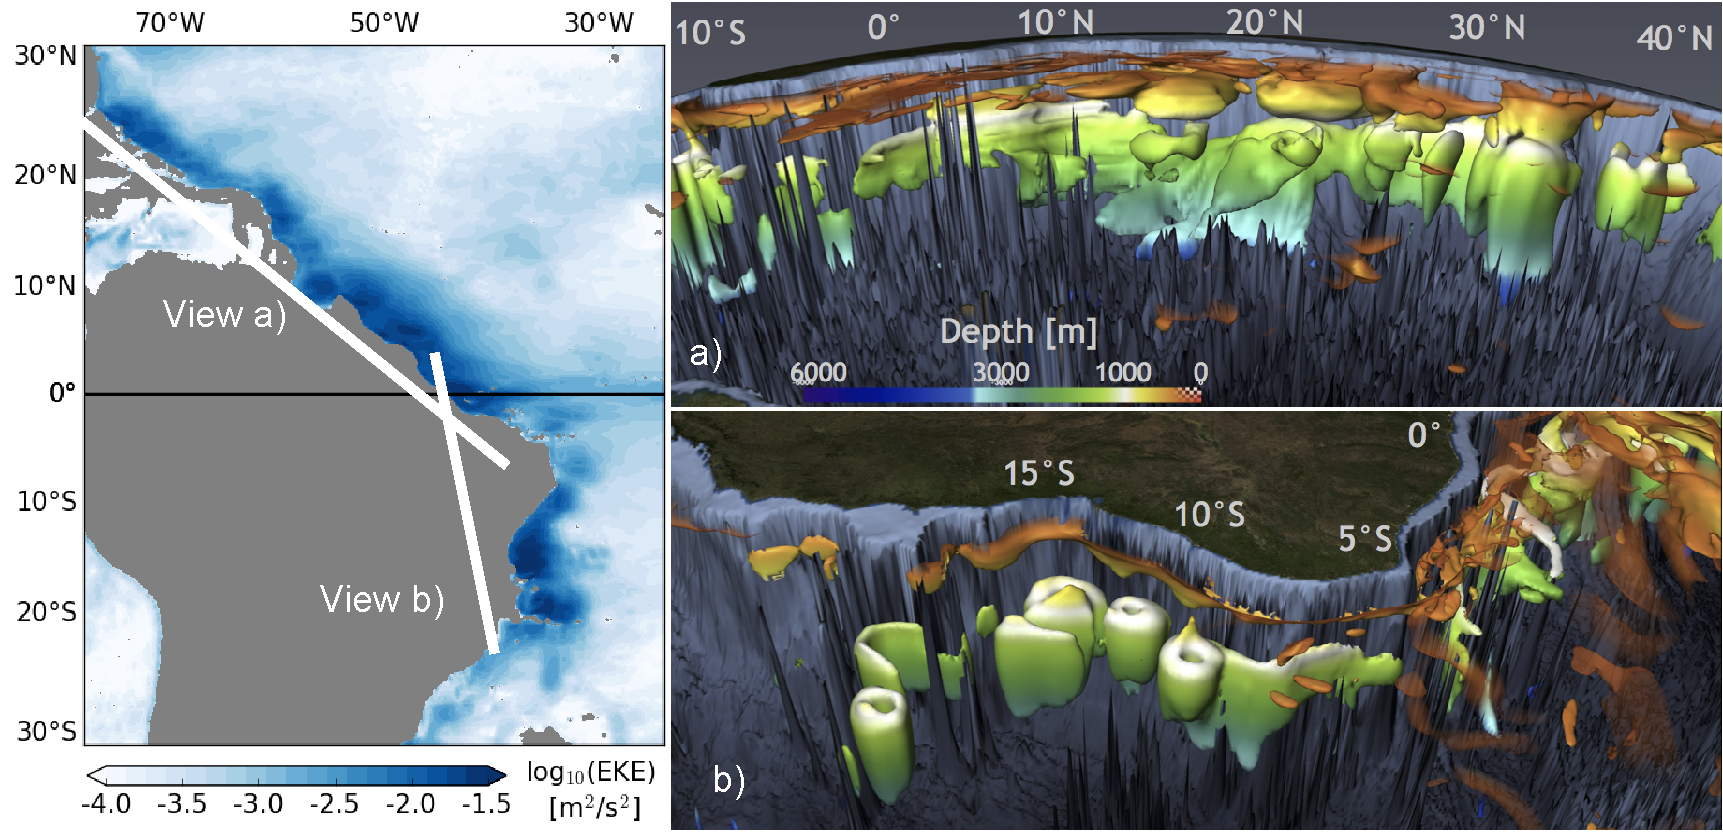
\includegraphics[width=0.99\textwidth]{figs/3D_and_map_.pdf}
\caption{\textbf{Left:} Eddy kinetic energy (EKE) in 1941 m depth in logarithmic color scale (blue contours). \textbf{Right:} 3D snapshots of the 0.2 m/s velocity magnitude contour surface. The color indicates depth, with white at 1000 m, where the DWBC begins (the colorbar is nonlinear). The flow above 400 m is made transparent as it would otherwise mask the DWBC. The angles of view of snapshot a) and b) are marked on the map in the left figure in white lines. }
\label{fig:eke_3D}
\end{figure}

\begin{figure}[t]\noindent
			\hspace{2.5mm}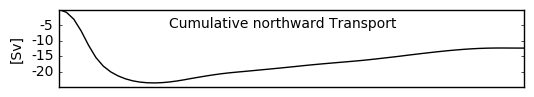
\includegraphics[width=24.4pc,angle=0]{figs/intro_DWBC_transport.png}\\
		
		\vspace*{-6mm}
	
		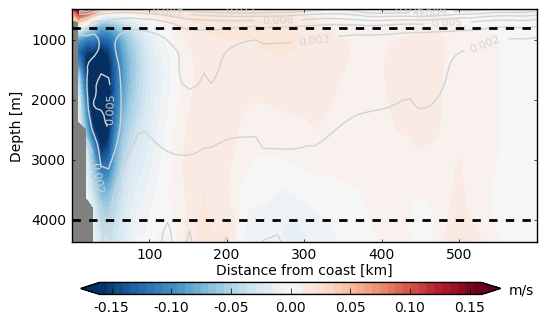
\includegraphics[width=25pc,angle=0]{figs/intro_DWBC_structure.png}\\
  \caption{(Top): STORM cumulative meridional transport of NADW between 800 m and 4000 m depth. The transport is computed from the western boundary eastwards. (Bottom): Meridional section along 26.5$^\circ$N. Meridional flow in colors (positive, red northwards).  Grey contour lines show eddy kinetic energy (EKE), the dashed lines define the layer of NADW, i.e. the area of DWBC transport relevant for the cumulative transport (top). }
\label{fig:intro_dwbc_structure}
\end{figure}


\begin{figure}
\label{fig:sketch_dwbc_north}
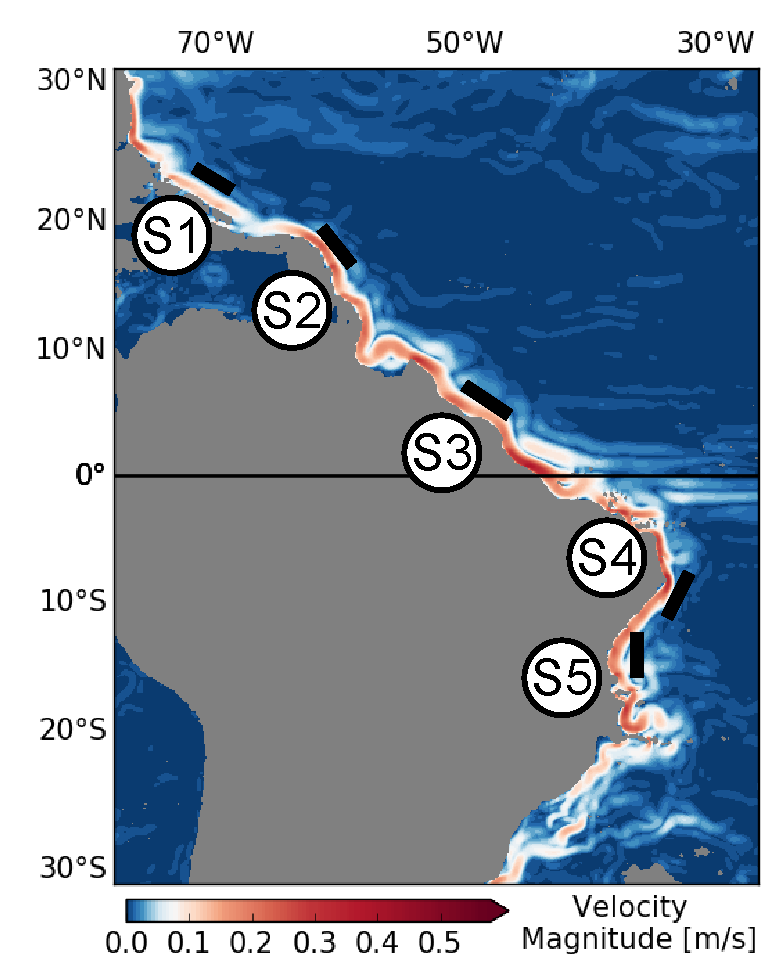
\includegraphics[height=8cm]{figs/blank_map_.pdf}
\caption{Mean flow velocity magnitude $|\mathbf{\overline u}|$ at 1941 m depth (non-linear color scale). The black bars depict the 5 DWBC segments (S1-S5) that we describe here.} 
\label{fig:segments}
\end{figure}


\begin{figure}[h!]
	\centering
	\begin{minipage}[]{0.32\textwidth}
	\centering S1: 23N-21N \\
		\center{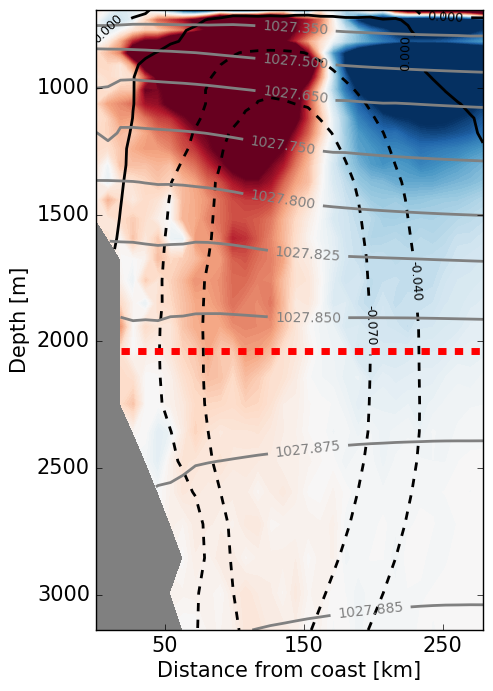
\includegraphics[height=7.cm]{figs/divUrho/divUrho23to21.png}} 
	\end{minipage}
%	\hfill
	\begin{minipage}[]{0.32\textwidth}
\centering S2: 16N-14N \\		
		\center{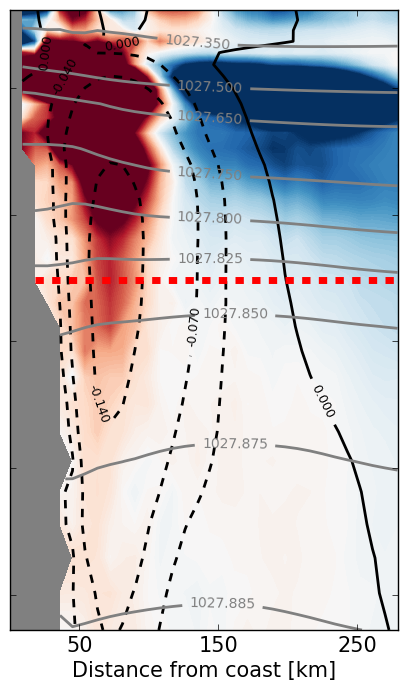
\includegraphics[height=7.cm]{figs/divUrho/divUrho16to14.png}} 
	\end{minipage}
	%	\hfill
	\begin{minipage}[]{0.32\textwidth}
\centering S3: 7N-5N \\		
		\center{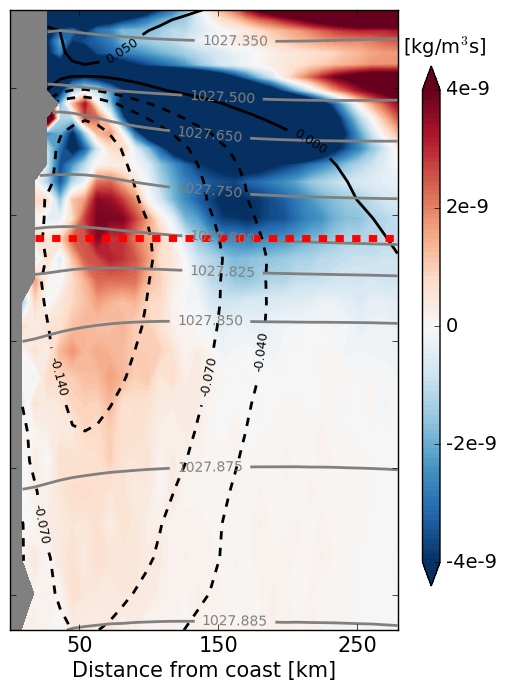
\includegraphics[height=7.cm]{figs/divUrho/divUrho7to5.png}} 
	\end{minipage}
		\caption{Pseudo-zonal sections of the along-stream average of the EDFD $\nabla \cdot (\overline{\mathbf{u'}\rho'})$ (colors), mean potential density $\overline{\rho}$ (gray contour lines) and along-stream flow $\mathbf{u_{||}}$ (black contour lines, dashed southwards) between 23$^\circ$N and 21$^\circ$N (left), 16$^\circ$N and 14$^\circ$N (center) and 7$^\circ$N and 5$^\circ$N (right). A positive (red) EDFD decreases and a negative (blue) EDFD increases density (note the minus sign in front of $\nabla \cdot (\overline{\mathbf{u'}\rho'})$ in Eq. \eqref{eq:density}). The red dashed line marks the DWBC core depth.}
\label{fig:results:EDFD_north}
\end{figure}

\begin{figure}
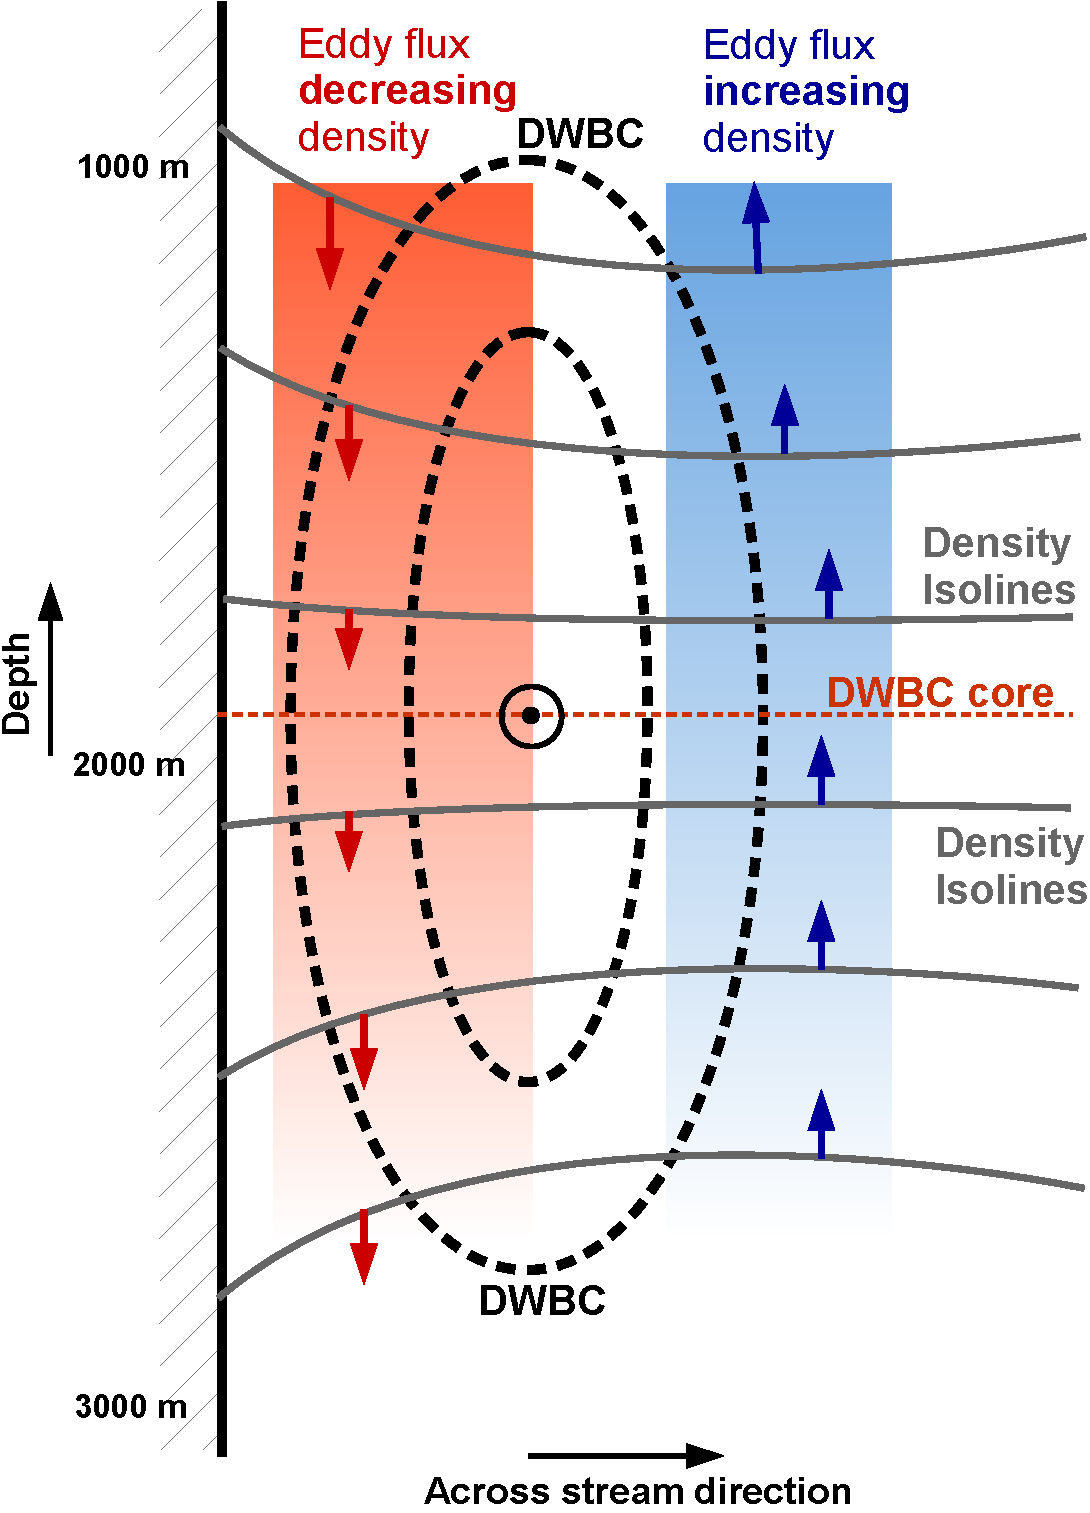
\includegraphics[height=7cm]{figs/sketch_north.pdf}\\
\caption{Sketch of Fig. \ref{fig:results:EDFD_north} that shows the EDFD (colors) and its relation to the isopycnals (gray contour lines) and along-stream velocity (black contour lines, dashed southwards). North of the equator, the EDFD \textit{decreases density close to the shore} (red patches here and in Fig. \ref{fig:results:EDFD_north})  and \textit{increases density further offshore} (blue patches here and in Fig. \ref{fig:results:EDFD_north}). A decrease of density causes a downward shift of the isopycnals (red arrows), whereas an increase causes an upward shift (blue arrows). Again, the red dashed line marks the DWBC core depth.} 
\label{fig:sketch_dwbc_north}
\end{figure}

\begin{figure}[h!]
	\centering
	\begin{minipage}[]{0.32\textwidth}
	\centering S4: 9S-11S \\
		\center{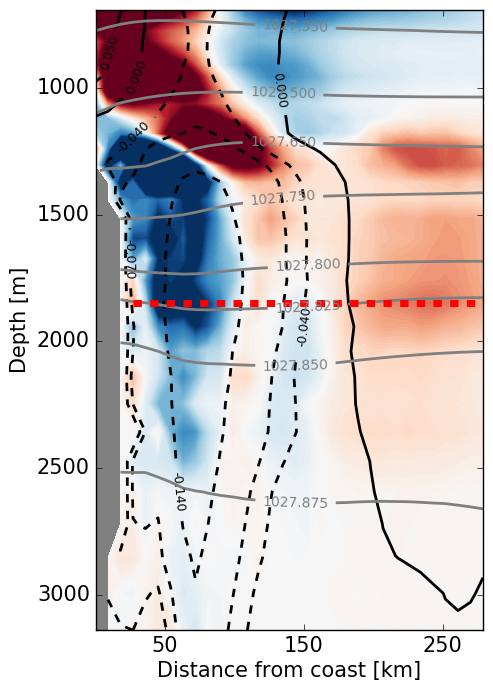
\includegraphics[height=7.cm]{figs/divUrho/divUrho-9to-11.png}} 
	\end{minipage}
	\begin{minipage}[]{0.32\textwidth}
\centering S5: 13S-15S \\		
		\center{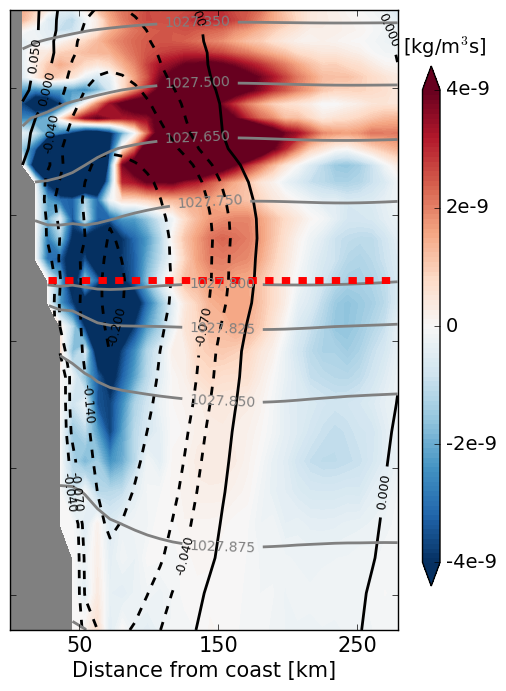
\includegraphics[height=7.cm]{figs/divUrho/divUrho-13to-15.png}} 
	\end{minipage}
	%\hfill
		\begin{minipage}[]{0.32\textwidth}
\centering Sketch South \\		
		\center{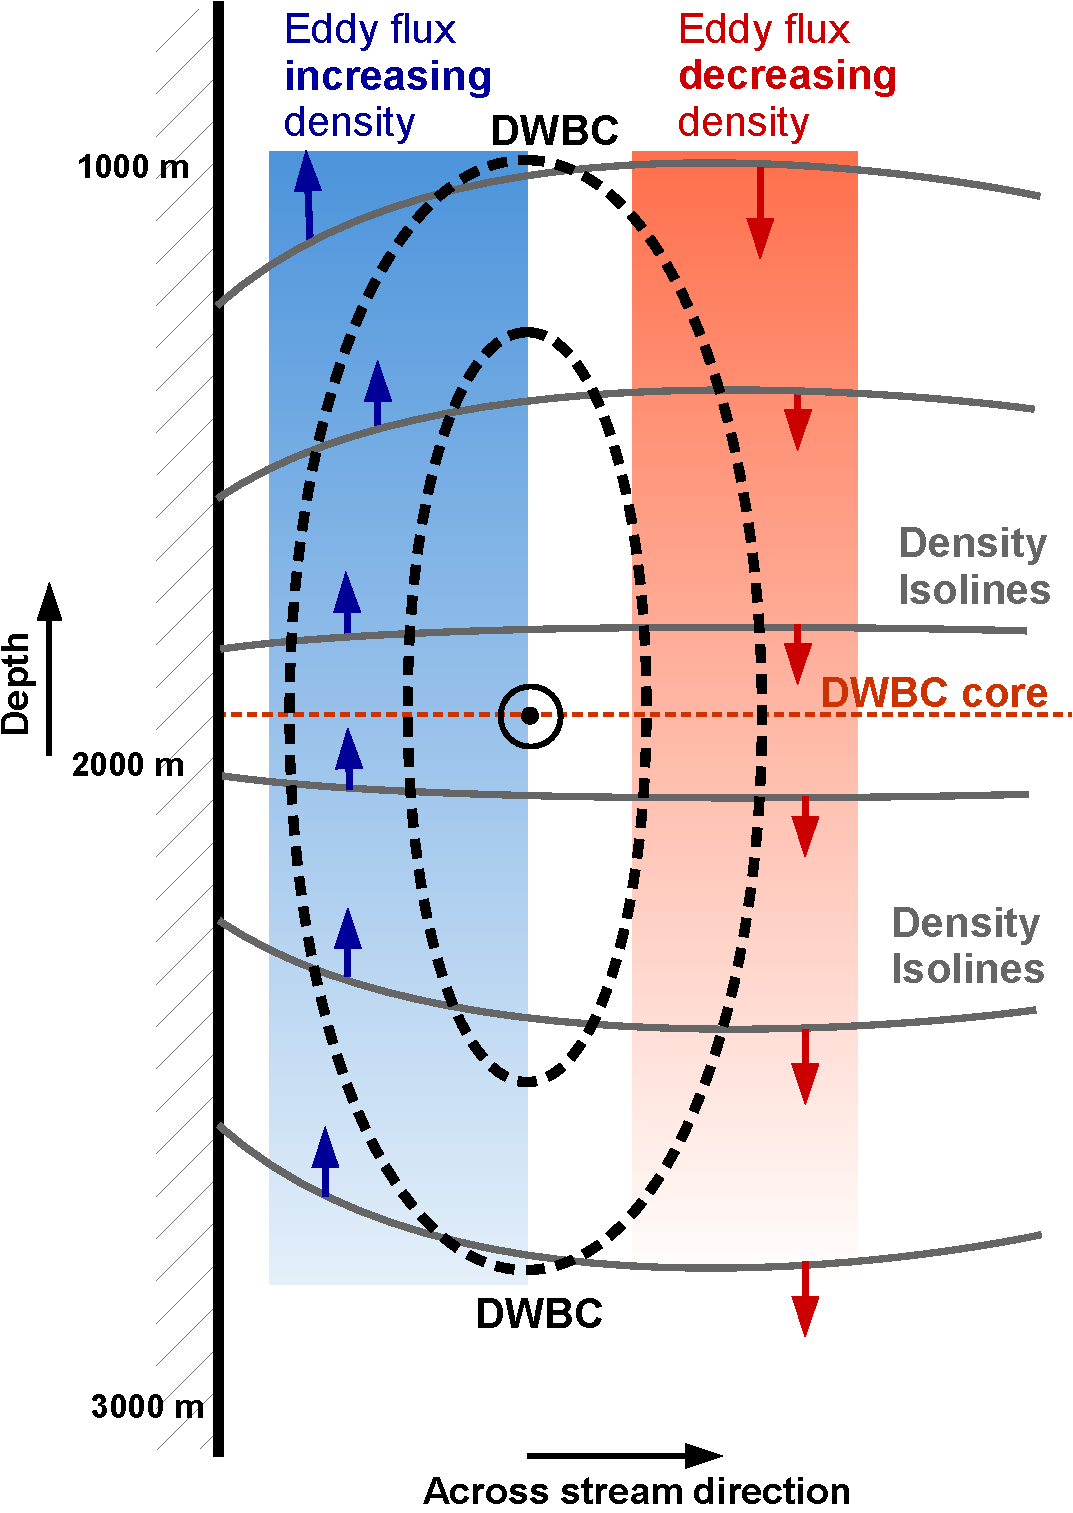
\includegraphics[height=7.cm]{figs/sketch_south.pdf}} 
	\end{minipage}
	\caption{Along-stream average of EDFD $\nabla \cdot (\overline{\mathbf{u'}\rho'})$ (colors), mean potential density $\overline{\rho}$ (gray contour lines) and along-stream flow $\mathbf{u_{||}}$ (black contour lines, dashed southwards) between 9$^\circ$S and 11$^\circ$S (left), 13$^\circ$S and 15$^\circ$S (center). The right panel shows a sketch similar to Fig. \ref{fig:sketch_dwbc_north} but for the southern hemisphere. }
		\label{fig:results:EDFD_south}
\end{figure}

\begin{figure}[h!]
	\centering
	\begin{minipage}[]{0.32\textwidth}
	\centering S1: 23N-21N \\
		\center{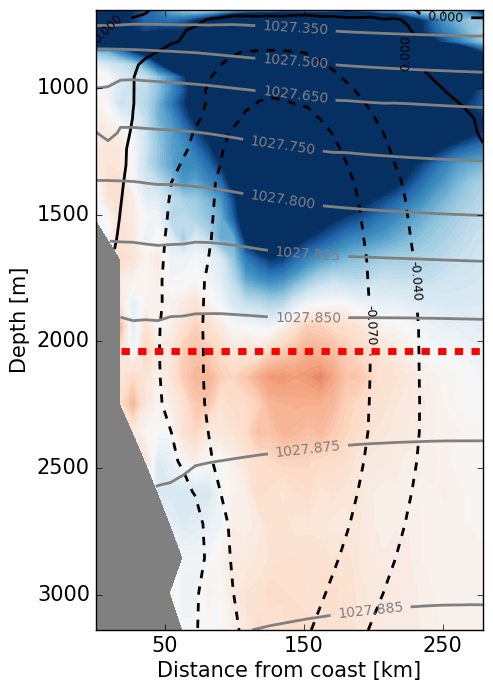
\includegraphics[height=7.cm]{figs/Pe2Pm/Pe2Pm23to21.png}} 
	\end{minipage}
	%\hfill
	\begin{minipage}[]{0.32\textwidth}
\centering S2: 16N-14N \\		
		\center{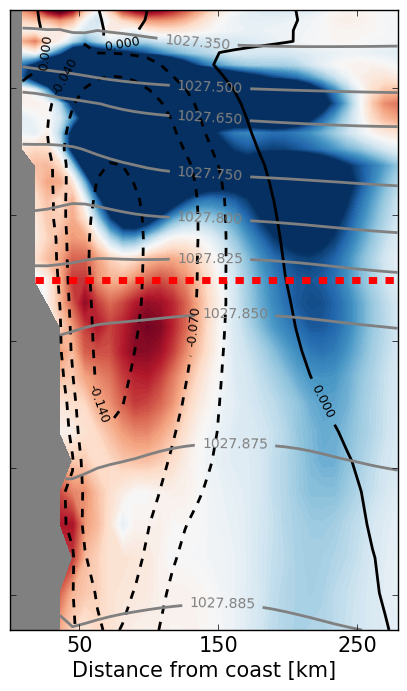
\includegraphics[height=7.cm]{figs/Pe2Pm/Pe2Pm16to14.png}} 
	\end{minipage}
	\begin{minipage}[]{0.32\textwidth}
\centering S3: 7N-5N \\		
		\center{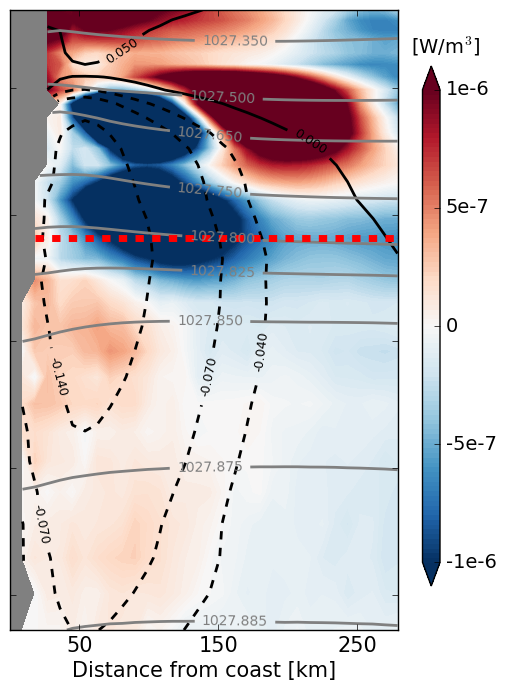
\includegraphics[height=7.cm]{figs/Pe2Pm/Pe2Pm7to5.png}} 
	\end{minipage}
	\caption{Like in Fig. \ref{fig:results:EDFD_north}, but the colors now indicate the along-stream averaged conversion from eddy potential energy to mean potential energy $\tilde{C}(\text{P}_\text{e},\text{P}_\text{m})$.}
	\label{fig:results:conversion_north}
\end{figure}

\begin{figure}[h!]
	\centering
	\begin{minipage}[]{0.32\textwidth}
	\centering S4: 9S-11S \\
		\center{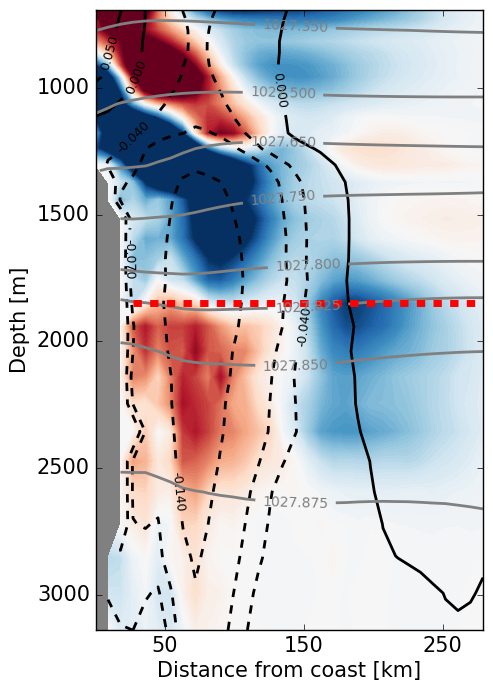
\includegraphics[height=7.cm]{figs/Pe2Pm/Pe2Pm-9to-11.png}} 
	\end{minipage}
	\begin{minipage}[]{0.32\textwidth}
\centering S5: 13S-15S \\		
		\center{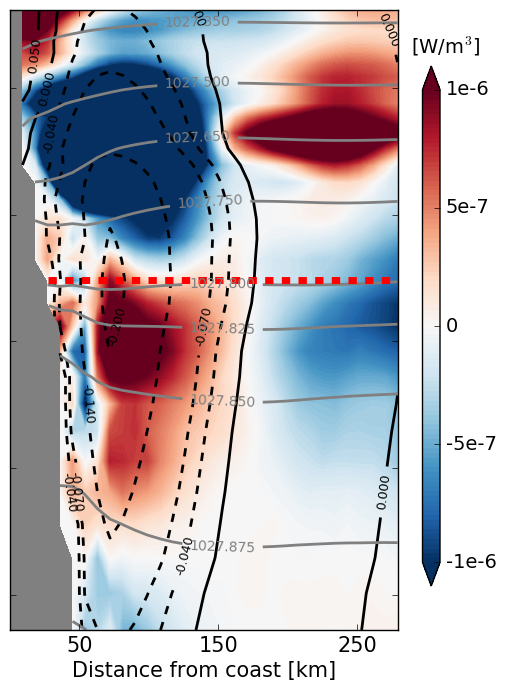
\includegraphics[height=7.cm]{figs/Pe2Pm/Pe2Pm-13to-15.png}} 
	\end{minipage}
	\caption{Like in Fig. \ref{fig:results:EDFD_south}, but the colors now indicate the along-stream averaged conversion from eddy potential energy to mean potential energy $\tilde{C}(\text{P}_\text{e},\text{P}_\text{m})$.}
		\label{fig:results:conversion_south}
\end{figure}

\begin{figure}[h!]
	\centering
	\begin{minipage}[]{0.32\textwidth}
	\centering S1: 23N-21N \\
		\center{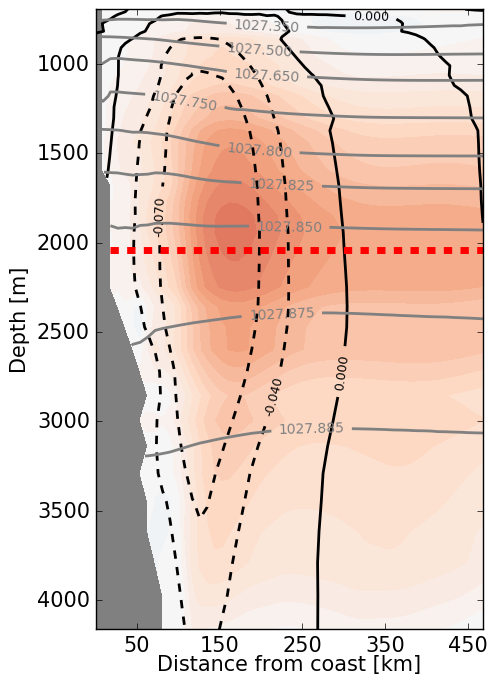
\includegraphics[height=7.cm]{figs/streamfunction/mean_streamfunction23to21.png}} 
	\end{minipage}
	%\hfill
	\begin{minipage}[]{0.32\textwidth}
\centering S2: 16N-14N \\		
		\center{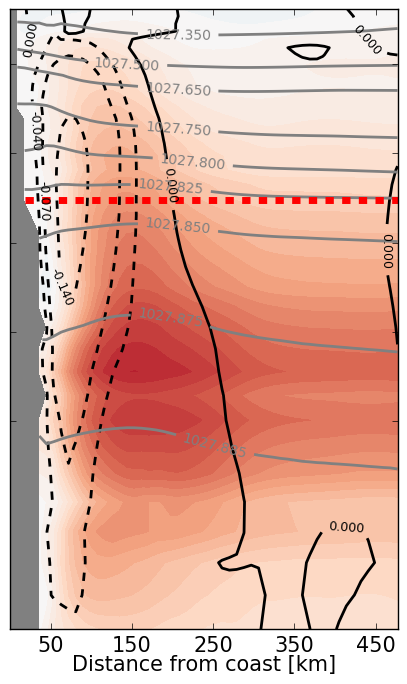
\includegraphics[height=7.cm]{figs/streamfunction/mean_streamfunction16to14.png}} 
	\end{minipage}
	\begin{minipage}[]{0.32\textwidth}
\centering S3: 7N-5N \\		
		\center{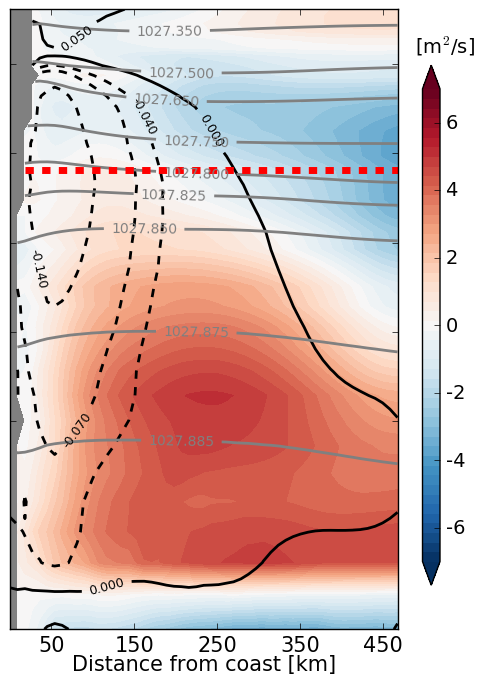
\includegraphics[height=7.cm]{figs/streamfunction/mean_streamfunction7to5.png}} 
	\end{minipage}
	\caption{Pseudo-zonal overturning per 1 m of shoreline $\Psi$ for the three segments north of the equator S1 (23$^\circ$N to 21$^\circ$N), S2 (16$^\circ$N to 14$^\circ$N) and S3 (7$^\circ$N and 5$^\circ$N). Positive (red) values indicate a clockwise overturning with upwelling close to the shore and downwelling further offshore. Again, the grey contour lines indicate potential density $\overline{\rho}$ and the black contour lines the along-stream flow $\overline{\mathbf{u_{||}}}$. The red dashed line marks the DWBC core depth.  }
	\label{fig:results:streamfunction_north}
\end{figure}

\begin{figure}[h!]
	\centering
	\begin{minipage}[]{0.32\textwidth}
	\centering S4: 9S-11S \\
		\center{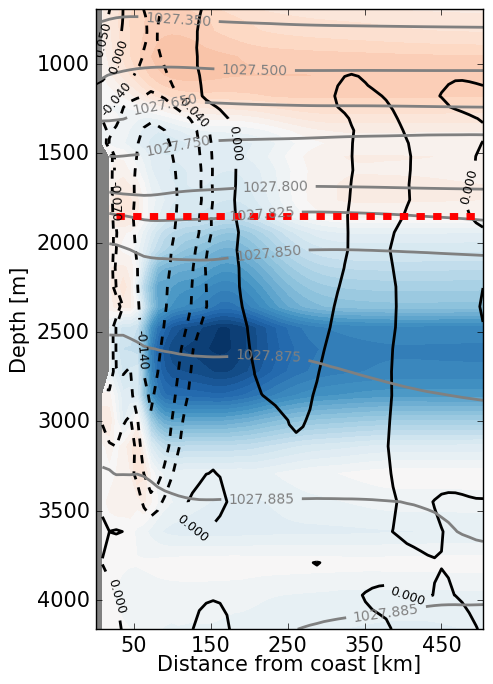
\includegraphics[height=7.cm]{figs/streamfunction/mean_streamfunction-9to-11.png}} 
	\end{minipage}
	\begin{minipage}[]{0.32\textwidth}
\centering S5: 13S-15S \\		
		\center{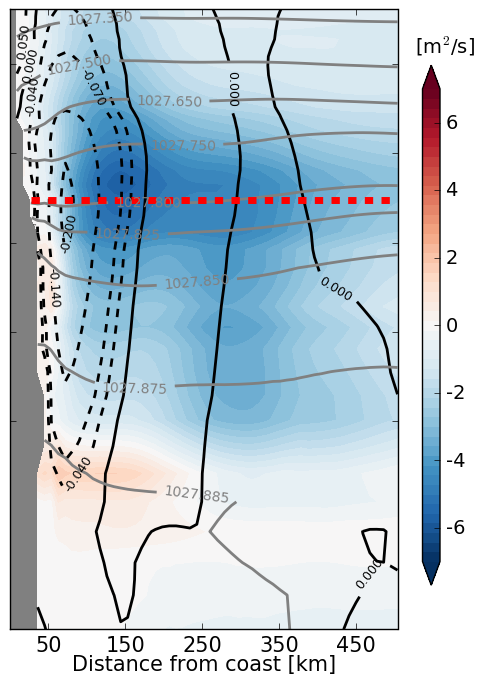
\includegraphics[height=7.cm]{figs/streamfunction/mean_streamfunction-13to-15.png}} 
	\end{minipage}
	\caption{Like in Fig. \ref{fig:results:streamfunction_north} but for the two segments south of the equator S4 (9$^\circ$S to 11$^\circ$S) and S5 (13$^\circ$S to 15$^\circ$S)}
		\label{fig:results:streamfunction_south}
\end{figure}

\end{document}